% The architecture diagram in the README. Rebuild docs/architecture.png from the
% repository root with
%   pdflatex -output-directory="$TMPDIR" docs/architecture.tex
%   pdftocairo -png -r 250 -singlefile "$TMPDIR/architecture.pdf" docs/architecture
\documentclass[tikz,border=12pt]{standalone}
\usepackage[T1]{fontenc}
\usepackage[scaled]{helvet}
\renewcommand{\familydefault}{\sfdefault}
\usepackage[none]{hyphenat}
\usetikzlibrary{positioning,fit,arrows.meta,backgrounds,calc,shapes.geometric}

% The application's own colours
\definecolor{accent}{HTML}{17607A}
\definecolor{accentsoft}{HTML}{E6F0F3}
\definecolor{ink}{HTML}{1F2A30}
\definecolor{muted}{HTML}{5B6B73}
\definecolor{lane}{HTML}{F4F7F8}
\definecolor{graph}{HTML}{B7791F}
\definecolor{graphsoft}{HTML}{FDF5E6}
\definecolor{mlflow}{HTML}{0194E2}

% The smaller grey line under a box's title
\newcommand{\sub}{\footnotesize\color{muted}}

\tikzset{
  every node/.style={text=ink},
  box/.style={draw=accent, line width=0.8pt, rounded corners=3pt, fill=white, align=center,
              inner sep=4pt, minimum height=12mm, text width=31mm, font=\small},
  io/.style={box, fill=accentsoft},
  note/.style={font=\footnotesize, text=muted},
  gnode/.style={draw=graph, line width=1.1pt, rounded corners=7pt, fill=white, align=center,
                minimum height=11mm, minimum width=23mm, font=\small},
  term/.style={draw=graph, line width=1.1pt, rounded corners=9pt, fill=graph!18,
               minimum height=8mm, minimum width=15mm, font=\footnotesize\ttfamily\bfseries},
  arr/.style={-{Stealth[length=2.4mm]}, line width=0.8pt, draw=ink!75},
  garr/.style={-{Stealth[length=2.4mm]}, line width=1pt, draw=graph},
  lbl/.style={font=\scriptsize\itshape, text=muted, fill=white, inner sep=1.5pt},
  lanebox/.style={fill=lane, draw=ink!15, rounded corners=6pt, inner sep=10pt},
  lanetitle/.style={font=\bfseries, anchor=north west},
}

\begin{document}
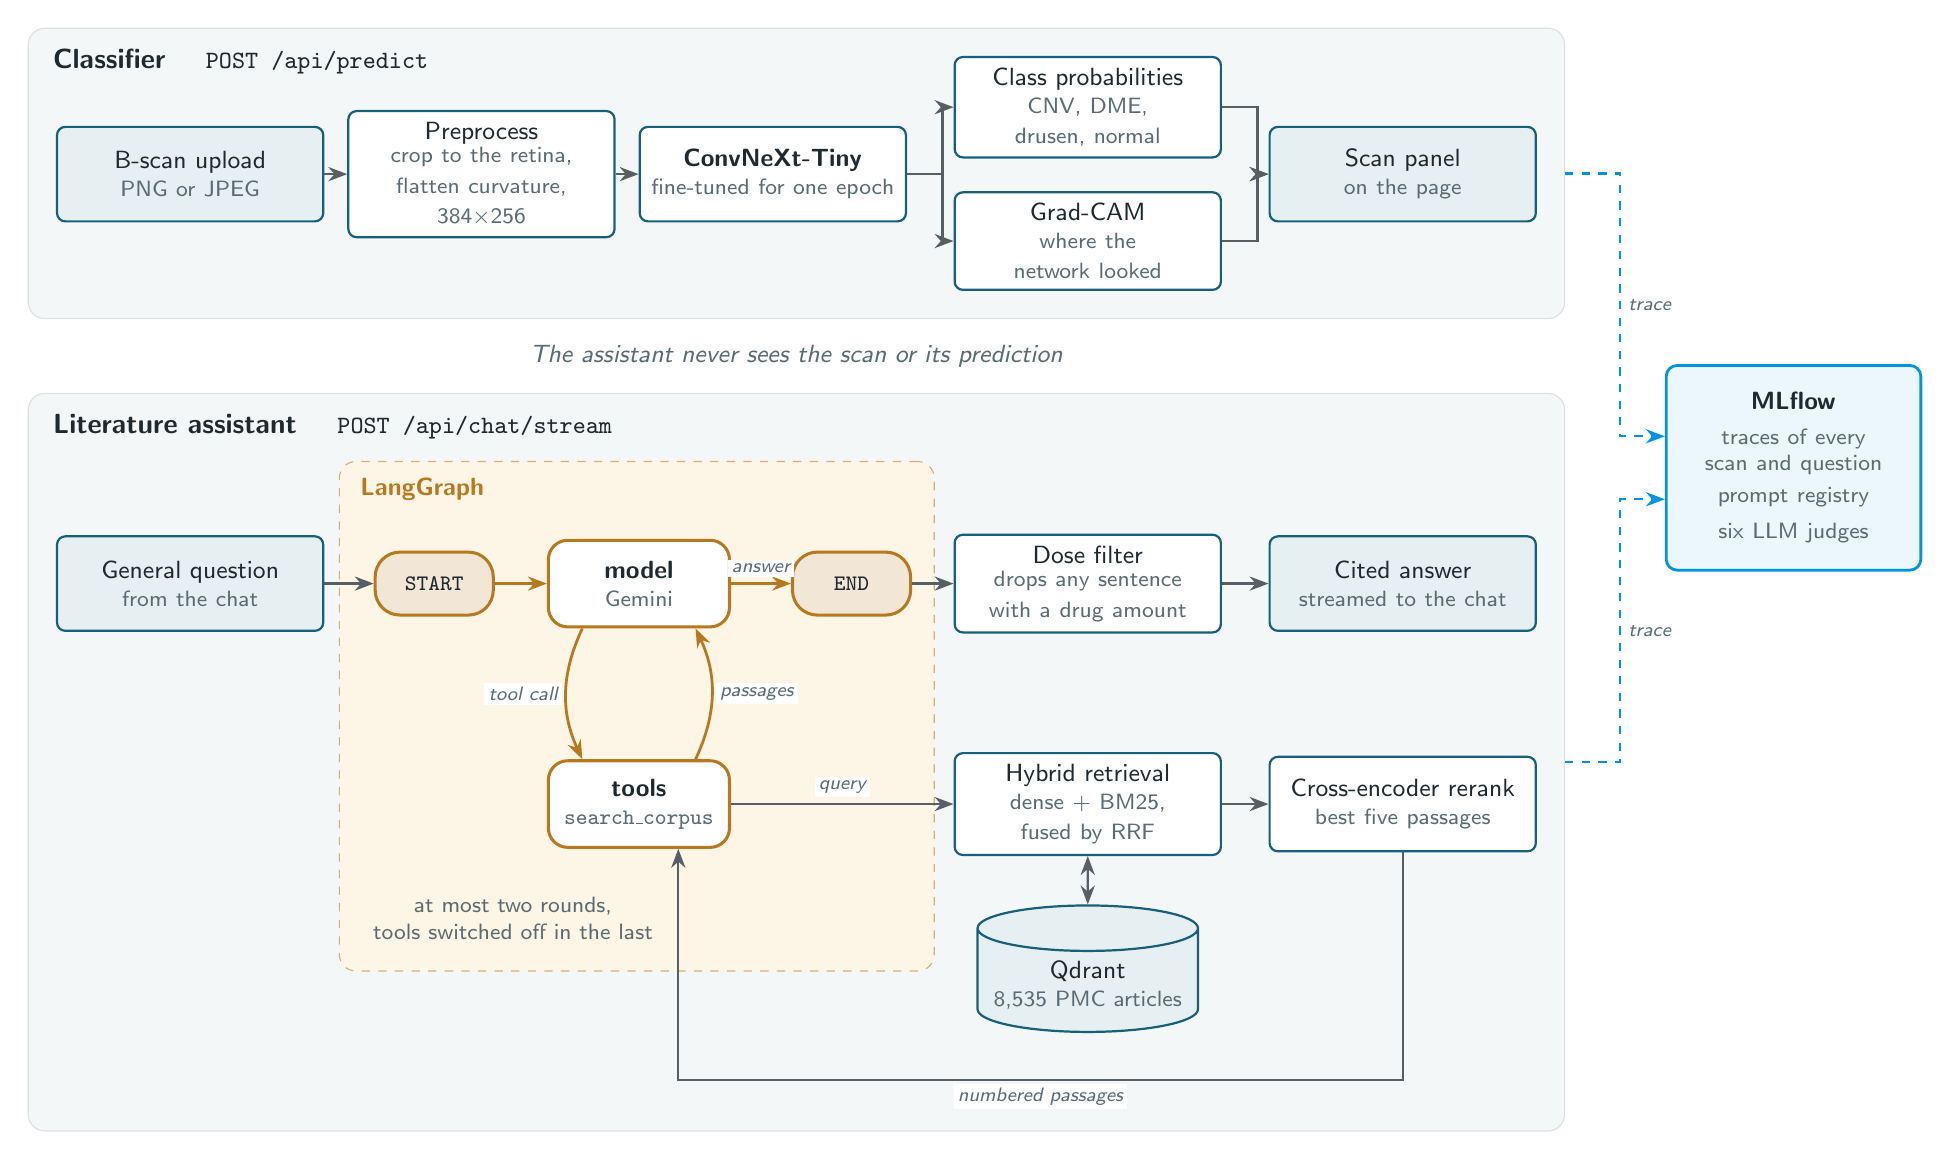
\begin{tikzpicture}

%% ---------------------------------------------------------------- classifier
\node[io]  (upload) at (0,0)     {B-scan upload\\[-1pt]{\sub PNG or JPEG}};
\node[box] (pre)    at (3.7,0)   {Preprocess\\[-1pt]{\sub crop to the retina,\\flatten curvature, 384$\times$256}};
\node[box] (cnn)    at (7.4,0)   {\textbf{ConvNeXt-Tiny}\\[-1pt]{\sub fine-tuned for one epoch}};
\node[box] (probs)  at (11.4,0.85) {Class probabilities\\[-1pt]{\sub CNV, DME, drusen, normal}};
\node[box] (cam)    at (11.4,-0.85) {Grad-CAM\\[-1pt]{\sub where the network looked}};
\node[io]  (scanui) at (15.4,0)  {Scan panel\\[-1pt]{\sub on the page}};

\draw[arr] (upload) -- (pre);
\draw[arr] (pre) -- (cnn);
\draw[arr] (cnn.east) -- ++(0.45,0) |- (probs.west);
\draw[arr] (cnn.east) -- ++(0.45,0) |- (cam.west);
\draw[arr] (probs.east) -- ++(0.45,0) |- (scanui.west);
\draw[arr] (cam.east) -- ++(0.45,0) |- (scanui.west);

%% ---------------------------------------------------------------- assistant
\node[io]   (q)     at (0,-5.2)    {General question\\[-1pt]{\sub from the chat}};
\node[term] (start) at (3.1,-5.2)  {START};
\node[gnode](model) at (5.7,-5.2)  {\textbf{model}\\[-1pt]{\sub Gemini}};
\node[gnode](tools) at (5.7,-8.0)  {\textbf{tools}\\[-1pt]{\sub\ttfamily search\_corpus}};
\node[term] (end)   at (8.4,-5.2)  {END};

\draw[arr]  (q) -- (start);
\draw[garr] (start) -- (model);
\draw[garr] (model.south west) ++(0.45,0) coordinate (ms)
            (ms) to[bend right=25] node[lbl, left=1pt] {tool call} ($(tools.north west)+(0.45,0)$);
\draw[garr] ($(tools.north east)+(-0.45,0)$) to[bend right=25] node[lbl, right=1pt] {passages}
            ($(model.south east)+(-0.45,0)$);
\draw[garr] (model) -- node[lbl, above=2pt] {answer} (end);

\node[box]  (dose)  at (11.4,-5.2) {Dose filter\\[-1pt]{\sub drops any sentence\\with a drug amount}};
\node[io]   (ans)   at (15.4,-5.2) {Cited answer\\[-1pt]{\sub streamed to the chat}};
\draw[arr] (end) -- (dose);
\draw[arr] (dose) -- (ans);

% the retrieval behind the tools node
\node[box] (hybrid) at (11.4,-8.0)  {Hybrid retrieval\\[-1pt]{\sub dense + BM25, fused by RRF}};
\node[box] (rerank) at (15.4,-8.0) {Cross-encoder rerank\\[-1pt]{\sub best five passages}};
\node[cylinder, shape border rotate=90, aspect=0.22, draw=accent, line width=0.8pt, fill=accentsoft,
      minimum width=28mm, minimum height=13mm, align=center, font=\small]
      (qdrant) at (11.4,-10.3) {Qdrant\\[-1pt]{\sub 8,535 PMC articles}};

\draw[arr] (tools) -- node[lbl, above=2pt] {query} (hybrid);
\draw[arr] (hybrid) -- (rerank);
\draw[arr, {Stealth[length=2.4mm]}-{Stealth[length=2.4mm]}] (hybrid) -- (qdrant);
% the passages go back to the tools node below Qdrant, so no line crosses it
\draw[arr] (rerank.south) -- (15.4,-11.5) -| node[lbl, pos=0.25, below=1pt] {numbered passages}
           ($(tools.south)+(0.5,0)$);

\node[note, align=center, text width=36mm] (rounds) at (4.1,-9.45)
     {at most two rounds,\\tools switched off in the last};

%% ---------------------------------------------------------------- lanes
% room above each lane's contents for its title
\coordinate (aTop) at ($(upload.north west)+(0,0.75)$);
\coordinate (bTop) at ($(q.north west)+(0,1.45)$);
\coordinate (bBot) at (0,-11.8);
\coordinate (gTop) at ($(model.north)+(0,0.7)$);
\begin{scope}[on background layer]
  \node[lanebox, fit=(upload)(probs)(cam)(scanui)(aTop)] (laneA) {};
  \node[lanebox, fit=(q)(qdrant)(ans)(rerank)(bTop)(bBot)] (laneB) {};
  \node[fill=graphsoft, draw=graph!60, dashed, rounded corners=6pt, inner sep=8pt,
        fit=(start)(model)(tools)(end)(gTop)(rounds)] (lg) {};
\end{scope}
\node[lanetitle] at ($(laneA.north west)+(0.2,-0.15)$) {Classifier \quad\mdseries\small\ttfamily POST /api/predict};
\node[lanetitle] at ($(laneB.north west)+(0.2,-0.15)$) {Literature assistant \quad\mdseries\small\ttfamily POST /api/chat/stream};
\node[font=\small\bfseries, text=graph, anchor=north west] at ($(lg.north west)+(0.15,-0.1)$) {LangGraph};

\node[font=\small\itshape, text=muted] at ($(laneA.south)!0.5!(laneB.north)$)
     {The assistant never sees the scan or its prediction};

%% ---------------------------------------------------------------- MLflow
\node[draw=mlflow, line width=1pt, rounded corners=4pt, fill=mlflow!8, align=center,
      text width=30mm, minimum height=26mm, font=\small]
      (mlflow) at ($(laneA.east)!0.5!(laneB.east)+(2.9,0)$)
      {\textbf{MLflow}\\[3pt]{\sub traces of every\\scan and question\\[2pt] prompt registry\\[2pt] six LLM judges}};
\draw[arr, dashed, draw=mlflow] (laneA.east) -- ++(0.7,0) |- node[lbl, pos=0.25, right=1pt] {trace} ($(mlflow.west)+(0,0.4)$);
\draw[arr, dashed, draw=mlflow] (laneB.east) -- ++(0.7,0) |- node[lbl, pos=0.25, right=1pt] {trace} ($(mlflow.west)+(0,-0.4)$);

\end{tikzpicture}
\end{document}
